\section{基于启发式算法的微电网日前经济调度优化}
\label{sec:economic_dispatch}

前文已针对光储充微电网系统在典型暂态工况下的物理动态响应与控制稳定性进行了详尽分析。在此基础上，从宏观的系统工程视角出发，微电网的完整运行体系不仅包含底层的暂态稳定，还需兼顾上层的长期稳态经济效益\upcite{ZGDL202303017}。由于底层电力电子设备的电磁暂态过程发生于毫秒至秒级，而上层能量管理系统的调度周期通常为小时级，两者在时间尺度上存在显著差异。因此，本章采用“时间尺度解耦”策略，忽略底层的瞬态高频波动，将研究重心转移至微电网的小时级能量管理与成本最优化。

本章将重点研究微电网的日前经济调度问题。旨在满足系统全局功率平衡与各项物理约束的前提下，通过合理安排储能系统的充放电计划以及与大电网的交互功率，实现微电网综合运行成本的最小化。本章首先建立微电网经济调度的数学模型，随后引入具有强大全局搜索能力的启发式算法（遗传算法或粒子群优化算法）对该非线性约束问题进行求解，最终通过典型日算例仿真验证优化调度策略的有效性。

\subsection{微电网日前经济调度数学模型}
\label{sec:math_model}

日前经济调度（Day-Ahead Economic Dispatch）的核心是在满足系统物理约束与负荷需求的前提下，以24小时为一个调度周期（通常划分为24个1小时的时段），优化计算各个时段储能系统的充放电功率与网侧交互功率\upcite{SJESBB7D5B55DB71628CEE2D751EFCBBEF5D}。

\subsubsection{目标函数}
本系统的综合运行成本目标函数 $F_{cost}$ 主要由三部分构成：与大电网的电能交互成本 $C_{grid}$、储能电池的寿命衰减折损成本 $C_{bat}$ 以及系统的日常运行维护成本 $C_{om}$。其数学表达式\upcite{GXXX202511001226}为：
\begin{equation}
    \min F_{cost} = \sum_{t=1}^{T} \left( C_{grid}(t) + C_{bat}(t) + C_{om}(t) \right) \Delta t
\end{equation}
式中，$T=24$ 为调度总时段数；$\Delta t=1\text{h}$ 为单次调度步长。

1. \textbf{电能交互成本}
\begin{equation}
    C_{grid}(t) = c_{buy}(t) P_{buy}(t) - c_{sell}(t) P_{sell}(t)
\end{equation}
式中，$c_{buy}(t)$ 与 $c_{sell}(t)$ 分别为 $t$ 时段的分时电价（TOU）购电与售电价格；$P_{buy}(t)$ 与 $P_{sell}(t)$ 分别为微电网向大电网购电与售电的功率。

2. \textbf{储能寿命衰减成本}
为对电池寿命进行评估，本节将第二章中建立的基于安时积分（Ah-throughput）的容量衰减经验模型引入经济调度中，将其量化为运行成本：
\begin{equation}
    C_{bat}(t) = K_{wear} |P_{bat}(t)|
\end{equation}
式中，$K_{wear}$ 为电池单次充放电循环的等效磨损惩罚系数；$P_{bat}(t)$ 为 $t$ 时段的电池吞吐功率。此项约束可有效防止算法为了赚取电价差价而导致电池过度频繁充放电。

3. \textbf{运行维护成本}
\begin{equation}
    C_{om}(t) = K_{pv} P_{pv}(t) + K_{c} |P_{bat}(t)|
\end{equation}
式中，$K_{pv}$ 与 $K_{c}$ 分别为光伏阵列与变流器的单位功率运维系数。

\subsubsection{约束条件}
在追求经济性最优的同时，系统调度必须严格遵守以下物理边界条件：

1. \textbf{全局功率平衡约束}
\begin{equation}
    P_{pv}(t) + P_{grid}(t) + P_{bat}(t) = P_{load}(t)
\end{equation}
式中，$P_{grid}(t) = P_{buy}(t) - P_{sell}(t)$ 为网侧净交互功率；$P_{load}(t)$ 为融合了蒙特卡洛模拟的电动汽车与常规负荷的总需求功率。

2. \textbf{储能系统约束}
为了防止电池深度过充过放，其荷电状态（SOC）与充放电功率必须被限制在安全区间：
\begin{equation}
    SOC_{min} \le SOC(t) \le SOC_{max}
\end{equation}
\begin{equation}
    -P_{bat}^{max} \le P_{bat}(t) \le P_{bat}^{max}
\end{equation}
同时，调度周期始末的 SOC 需保持一致，以保证跨日调度的可持续性：$SOC(0) = SOC(T)$。

3. \textbf{并网交互功率约束}
\begin{equation}
    -P_{tie}^{max} \le P_{grid}(t) \le P_{tie}^{max}
\end{equation}
式中，$P_{tie}^{max}$ 为并网联络线的最大物理传输容量。

\subsection{基于粒子群优化算法的模型求解}
\label{sec:pso_algorithm}

微电网日前经济调度本质上是一个多变量、多约束的非线性连续优化问题。遗传算法（GA）等传统启发式算法在处理此类问题时常需要复杂的二进制编码与解码过程，计算效率受限。因此，本章采用粒子群优化算法（Particle Swarm Optimization, PSO）进行求解。PSO 算法源于对鸟群觅食行为的模拟，具有参数少、易于实现且对连续实数空间寻优能力强的显著优势，极其契合本文连续功率调度的需求\upcite{SJPD0C4BE4F85220580A31E7677AEF821B45}。

\subsubsection{PSO 算法基本原理}
在 PSO 算法中，每一个潜在的调度方案（即 24 小时的储能充放电功率序列）被抽象为多维搜索空间中的一个“粒子”。设搜索空间为 $D$ 维，种群规模为 $N$。第 $i$ 个粒子的位置系列表示为 $X_i = (x_{i1}, x_{i2}, ..., x_{iD})$，其飞行速度表示为 $V_i = (v_{i1}, v_{i2}, ..., v_{iD})$。

在每次迭代中，粒子根据自身历史找到的最优位置（个体极值 $P_{best}$）和整个种群找到的最优位置（全局极值 $G_{best}$）来动态更新自身的速度与位置\upcite{SJMD1888C91A0619D8337CB2AAFCC2DBF6D7}。其核心迭代方程如下：

\begin{equation}
    v_{id}^{k+1} = \omega v_{id}^k + c_1 r_1 (p_{best,id}^k - x_{id}^k) + c_2 r_2 (g_{best,d}^k - x_{id}^k)
\end{equation}

\begin{equation}
    x_{id}^{k+1} = x_{id}^k + v_{id}^{k+1}
\end{equation}

式中：$k$ 为当前迭代次数；$v_{id}$ 与 $x_{id}$ 分别为粒子 $i$ 在第 $d$ 维的速度与位置；$\omega$ 为惯性权重，用于平衡算法的全局与局部搜索能力；$c_1, c_2$ 为学习因子（加速常数），代表粒子向自身经验和群体经验学习的权重；$r_1, r_2$ 为 $[0,1]$ 之间均匀分布的随机数。

\subsubsection{算法求解流程}
针对本文的微电网调度模型，PSO 算法的具体求解步骤如下：
\begin{enumerate}
    \item \textbf{参数初始化}：设定粒子群规模 $N$、最大迭代次数 $K_{max}$、学习因子 $c_1, c_2$ 及惯性权重 $\omega$。随机初始化粒子的位置（24小时的电池功率分配）与速度。
    \item \textbf{适应度评估}：将每个粒子的位置代入 4.1 节构建的综合运行成本目标函数中计算适应度值。对于违反 SOC 上下限或功率交互约束的粒子，施加极大的罚函数（Penalty Function）予以淘汰。
    \item \textbf{极值更新}：比较当前适应度与历史最优适应度，更新每个粒子的 $P_{best}$；比较全群粒子的适应度，更新种群的 $G_{best}$。
    \item \textbf{状态迭代}：根据速度与位置更新公式，计算下一代粒子的飞行状态。
    \item \textbf{终止条件判断}：若达到最大迭代次数 $K_{max}$ 或连续多代全局最优解变化小于设定阈值，则终止寻优并输出 $G_{best}$ 作为最终的日前最优经济调度策略；否则返回步骤 2 继续迭代。
\end{enumerate}

\subsection{日前经济调度仿真结果与分析}
\label{sec:dispatch_results}

为验证所提基于 PSO 算法的微电网日前经济调度策略的有效性，本文在 MATLAB 环境中编写了寻优算法脚本。系统设定调度周期为 24 小时，步长为 1 小时。算法种群规模设为 300，最大迭代次数为 500 次。考虑到微电网的实际物理限制，特别在目标函数中引入了针对电池频繁充放电切换的严厉惩罚项，以避免产生损害电池寿命的高频震荡策略。仿真优化结果如图 \ref{fig:pso_results} 所示。

\begin{figure}[htbp]
    \centering
    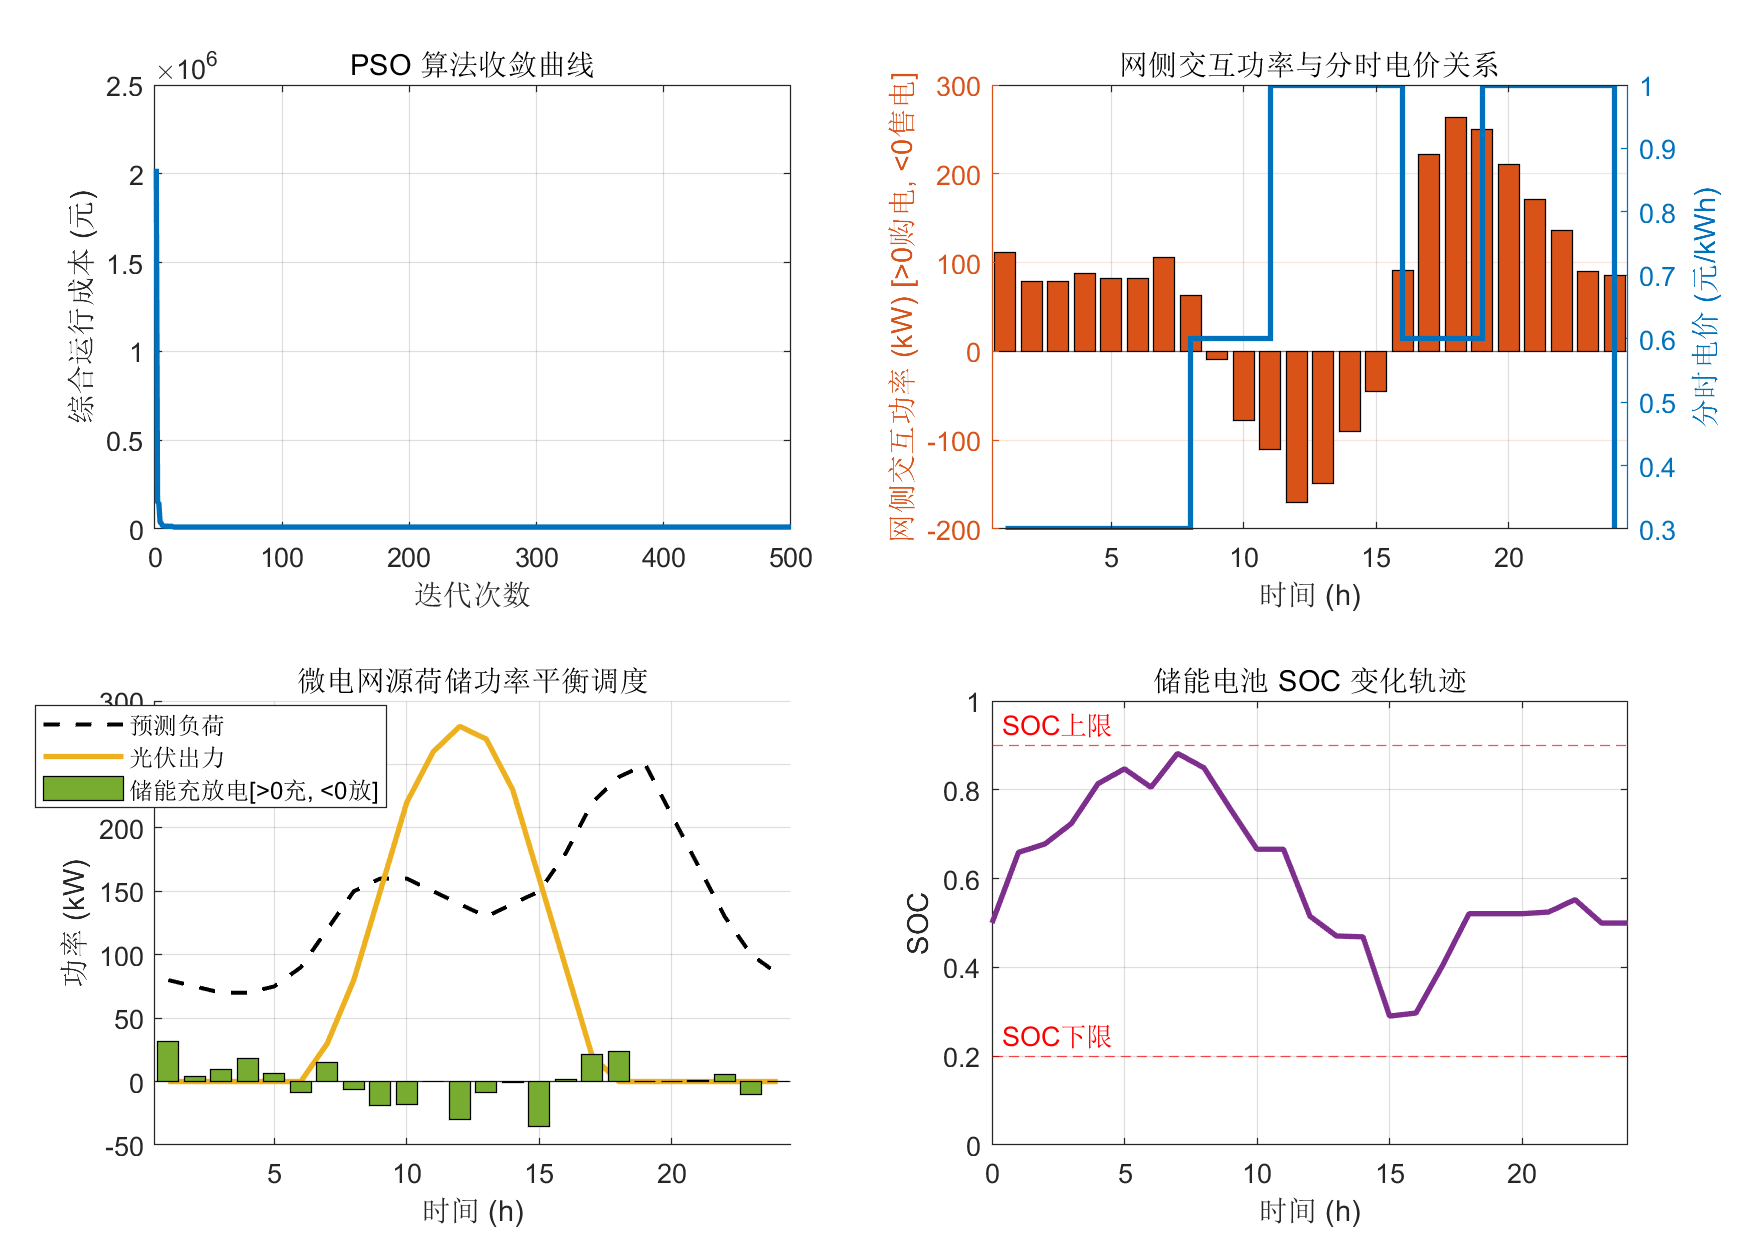
\includegraphics[width=0.9\textwidth]{figures/fig4_1_pso_results.png}
    \caption{微电网日前经济调度综合优化结果}
    \label{fig:pso_results}
\end{figure}

由图 \ref{fig:pso_results} 中“PSO 算法收敛曲线”可知，算法在迭代初期迅速找到了一个较低的成本可行解，并在后续的迭代过程中，得益于惯性权重的自适应递减机制，粒子群在局部空间内进行了精细的微调探索，最终收敛于全局最优解，充分验证了算法的高效性与稳定性。

结合“网侧交互功率与分时电价关系”及“微电网源荷储功率平衡调度”两图可以清晰地观察到储能系统的套利行为逻辑：在凌晨（01:00-07:00）的谷电价时段，系统主要依靠大电网供电，同时储能电池在此期间进行平稳、连续的充电以储备廉价电能；在日间（10:00-15:00），随着光伏出力的达到顶峰，微电网不仅实现了自给自足，还将冗余的清洁电能售卖给大电网以获取经济收益；而在傍晚至夜间（18:00-23:00）的光伏出力低谷及峰电价时段，储能电池转入连续放电模式，极大地削减了系统向大电网高价购电的需求\upcite{SJESBE9A2800B7786FFCC006B629BFBD8D48}。

值得注意的是，在引入了防震荡惩罚机制后，储能电池的充放电策略呈现出高度的平滑性与连续性，彻底消除了无意义的频繁充放电跳变。从“储能电池 SOC 变化轨迹”图中可以看出，电池的 SOC 严格约束在 $[0.2, 0.9]$ 的安全边界内。更为关键的是，调度周期末端（第 24 小时）的 SOC 完美回落至初始值 $0.5$，这一精准的闭环特性不仅保证了跨日调度的可持续性，更在宏观时间尺度上有效延缓了电池容量的衰减，实现了系统经济性与设备寿命的双赢。

\subsection{本章小结}
本章从微电网的宏观经济运行视角出发，重点研究了基于粒子群优化（PSO）算法的光储充电站日前经济调度策略。首先，建立了以微电网综合运行成本最小化为目标的数学模型，该模型全面考虑了电网分时电价（TOU）套利、储能电池充放电折损成本以及各项物理功率边界约束。其次，针对微电网多变量连续优化的特点，引入了PSO算法进行求解，并创新性地在适应度函数中加入了防震荡与SOC闭环惩罚机制。最后，通过MATLAB算例仿真验证了所提策略的有效性。仿真结果表明，该调度策略能够引导系统在谷电价时段储能、峰电价时段放电售电，不仅有效实现了电网的削峰填谷，显著降低了微电网的日均运行成本，还严格保障了储能电池的安全运行与寿命健康，圆满完成了微电网系统级的优化运行目标。